\documentclass{ximera}

\newcommand{\RR}{\mathbb R}
\renewcommand{\d}{\,d}
\newcommand{\dd}[2][]{\frac{d #1}{d #2}}
\renewcommand{\l}{\ell}
\newcommand{\ddx}{\frac{d}{dx}}
\newcommand{\dfn}{\textbf}
\newcommand{\eval}[1]{\bigg[ #1 \bigg]}


\author{Jim Talamo and Alex Beckwith}
\license{Creative Commons 3.0 By-NC}


\outcome{Set up an integral that gives the length of a curve segment and evaluate it}

\begin{document}
\begin{exercise}

A cylindrical tank has base diameter 10m and height 6m. Suppose the tank is filled halfway with water ($\rho$=1000 kg/m$^3$). Find the work required to pump the water out of the tank (use $g=9.8$m/s$^2$).
\begin{image}
	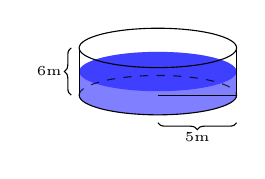
\begin{tikzpicture}
	
	\fill [blue,opacity=0.5] (0,-0.3) ellipse (1 and 0.25);
	\fill [blue,opacity=0.5] (-1,-0.3) -- (-1,-0.6) arc (180:360:1 and 0.25) -- (1,-0.3) arc (0:180:1 and 0.25);
	
	\draw (0,0) ellipse (1 and 0.25);
	\draw (-1,0) -- (-1,-0.6);
	\draw (-1,-0.6) arc (180:360:1 and 0.25);
	\draw [dashed,opacity=0.75] (-1,-0.6) arc (180:360:1 and -0.25);
	\draw (1,-0.6) -- (1,0);  
	\draw (0,-0.6) -- (1,-0.6); 
	
	\draw[decoration={brace,raise=.1cm},decorate,thin] (-1,-0.6) -- (-1,0);
	\node[anchor=east] at (-1.1,-0.3) {\tiny $6$m};
	
	\draw[decoration={brace,raise=.1cm},decorate,thin] (1,-0.85) -- (0,-0.85);
	\node[anchor=north] at (.5,-0.95) {\tiny $5$m};

	\end{tikzpicture}
\end{image}

\[
W= \int_{y=\answer{0}}^{y=\answer{3}}  \answer{245000\pi (6-y)}\d y = \answer[tolerance=10]{3307500\pi} J
\]

\begin{hint}
To check your work: 

$\rho g = \answer{9800}$

$A(y) = \answer{25 \pi}$
\end{hint}

\end{exercise}
\end{document}
